\subsection{Differential gears}

Differential gears are used to reduce slipping between opposite wheels when the vehicle is turning. The system can not avoid slipping under the tracks because they are too long, they will rotate at least around the center of the track. However, using differential gears will help control the course of the vehicle by braking one of the tracks and transfering some of it's power to the other track.\\

The system of differential gears is simple. As seen on \figref{pinion-ring-spider_gear}, the power is transmitted from the pinion gear to the spider gear fixed on the ring gear. Only the spider gear is connected to the side gears, fixed to the wheels, as seen on the \figref{full_differential_gears}. When the ring gear is turning but the spider gear does not spin, both side gear turn the same speed, but if the spider gear spins also, one side gear will turn faster than the other.\\

This is the element the servo is using when braking one track, allowing the other track to turn independently, with even more speed because the power remaining will go on the power free side gear.\\


\begin{figure}[H]
	\centering
	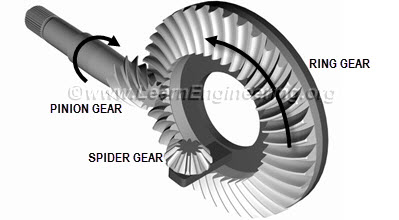
\includegraphics[scale=1]{figures/pinion-ring-spider_gear.jpg}
	\caption{Transfer of the power to the spider gear}
	\label{pinion-ring-spider_gear}
\end{figure}
\todo{insert source}
%http://www.learnengineering.org/2014/05/working-of-differential.html

\begin{figure}[H]
	\centering
	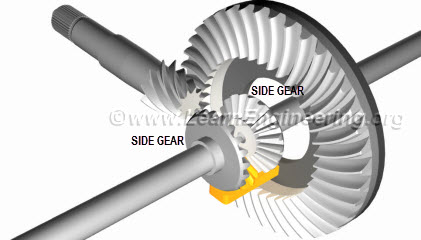
\includegraphics[scale=1]{figures/full_differential_gears.jpg}
	\caption{transfer of the power to the side wheels}
	\label{full_differential_gears}
\end{figure}
\todo{insert source}
%http://www.learnengineering.org/2014/05/working-of-differential.html
